\section{Underlying modeling technique (0.5 pages)}
\label{section:contribution_0}

Our approach is based on emergent property estimation techniques \cite{hackenberg2012towards} and uses a model-based approach for validating requirements in early phases of development proposed in \cite{hackenberg2014rapid}, relying on partial system models to ease modeling effort. An adaption to the ITS domain of this modeling technique was proposed in \cite{ascher2014early}, facilitating the formulation of multi-objective traffic flows as an optimal control problem consisting of state variables, control variables, constraints and objectives. The approach employs a generic solver for system behavior estimation, which utilizes stochastic optimization techniques.

\begin{figure}[h]
	\centering
	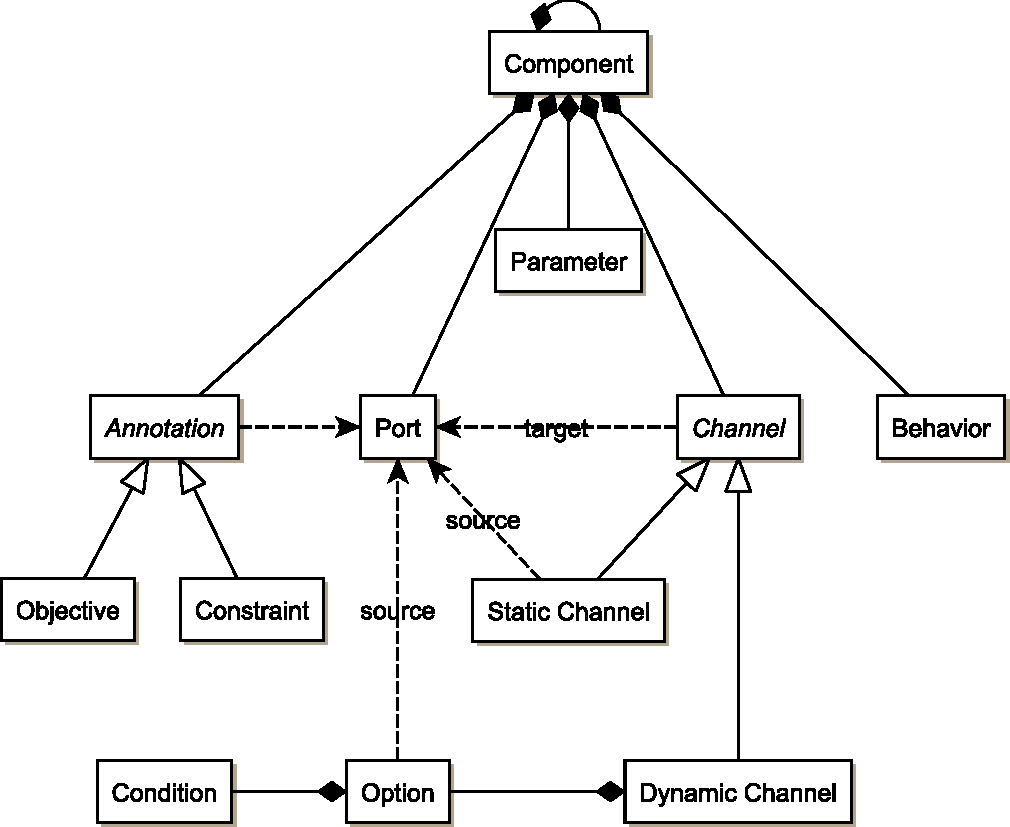
\includegraphics[width=\columnwidth]{../gfx/meta_model.pdf}
	\caption{Meta-model.}
	\label{fig:model}
\end{figure}

In terms of their structure, model components can be atomic or can be composed by other components. Model components have a set of input and output ports, which represent observations about specific behavior. Directed connections between ports allow the modeling of interactivity between different components.

\section{Holistic parametric approach (3 pages)}
\label{section:contribution_1}

In our approach, model definition is aided by a composite model architecture fitted to transportation scenario modeling seen in Figure~\ref{fig:model}. On it's highest level, the model architecture is represented by the system model, which contains separate models for the traffic and the power system. The traffic model represents the traffic system, in which individual cars within the traffic infrastructure are contained. Similarly, the power model represents the power system, which is comprised of different energy producing or energy consuming power devices, such as solar panels, energy storages and charging stations. Furthermore, the power system includes the electricity infrastructure such as low-voltage nets and medium-voltage nets.

\begin{figure*}[h]
	\centering
	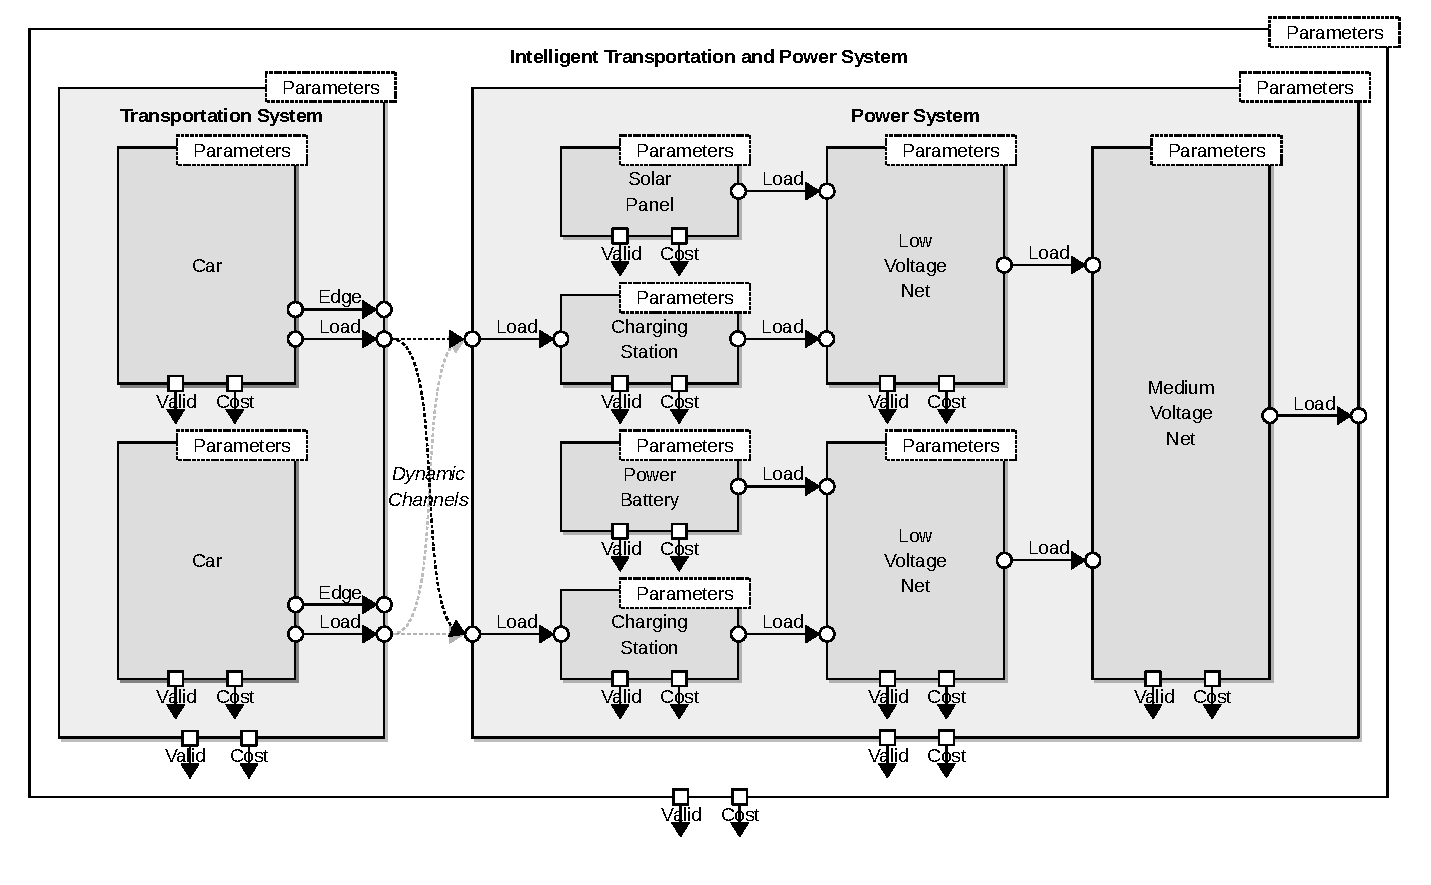
\includegraphics[width=\textwidth]{../gfx/model2.pdf}
	\caption{Overview of the multi-domain system modeling approach including the transportation system and the power system.}
	\label{fig:model}
\end{figure*}

The holistic parametric approach allows for each component to be initialized using a specific set of parameters. Subsequently we describe the different components of the model architecture in terms of their respective parameters, interface, structure and behavior. 

\subsection{Intelligent Transportation and Power System}
On it's highest level, the model architecture is represented by the system model, which contains separate models for both mandatory traffic and power systems.

	 \begin{table}[h]
	 	\renewcommand{\arraystretch}{1.3}
	 	\caption{Transportation System Component Parameters}
	 	\centering
	 	\begin{tabular}{lll}
	 		\hline
	 		\textbf{Parameter}                    & \textbf{Unit} & \textbf{Description} \\ \hline
	 		Traffic Network                  	  & Graph          & Graph of the traffic network      \\
	 		Transportation System                 & Component    & Contained transportation system    \\ 
	 		Power System                 		  & Component   & Contained power system    \\ \hline
	 	\end{tabular}
	 \end{table}
	 \begin{itemize}
	\item Interface: 
			\begin{itemize}
				\item Inputs: Power System Load, Power System Cost, Transportation System Cost
				\item Outputs: Cost, Validity, Balance
			\end{itemize}	
	\item Structure: Component, which is composed of power system and transportation system component.
	\item Behavior: The intelligent transportation and power system aggregates the costs of the power system and the transportation system, which it contains, and defines a minimization objective function on these costs:
	Furthermore, it gathers the total energy balance from the power system.
\end{itemize}


\subsection{Transportation System}

The transportation contains the traffic infrastructure, i.e. traffic network,  as well as the individual cars on the traffic infrastructure.

	 \begin{table}[h]
	 	\renewcommand{\arraystretch}{1.3}
	 	\caption{Transportation System Parameters}
	 	\centering
	 	\begin{tabular}{lll}
	 		\hline
	 		\textbf{Parameter}                    & \textbf{Unit} & \textbf{Description} \\ \hline
	 		Traffic Network                  	  & Graph          & Graph of the traffic network      \\
	 		Number of Cars                          & Numeral    & Number of cars      \\ 
	 		Car Type Distribution                          & Numeral[]    & Distribution of different car types      \\ 
	 		Car                          & Component[]    & Contained car components      \\ \hline
	 	\end{tabular}
	 \end{table}
	 \begin{itemize}
	\item Interface:
			\begin{itemize}
				\item Inputs: Car Component Costs
				\item Outputs: Transportation System Cost, Transportation System Validity
			\end{itemize}	 
	\item Structure: Component, which is composed of car components.
	\item Behavior: The transportation system aggregates the costs of the individual car components it contains. Furthermore, the transportation system implements a constraint on the car components which tests if cars overlap each other on their respective current positions.
\end{itemize}

\subsection{Car}

Cars can alternately act as energy producers, consumers and storages by charging or discharging at charging stations.

	 \begin{table}[h]
	 	\renewcommand{\arraystretch}{1.3}
	 	\caption{Car Parameters}
	 	\centering
	 	\begin{tabular}{lll}
		 	\hline
			\textbf{Parameter}                    & \textbf{Unit} & \textbf{Description} \\ \hline
			Origin                                & Edge          & Origin Position      \\
			Destination                           & Edge          & Destination Position \\
			State of Charge Weight                & Numeral       & Weight of the state of charge objective                     \\
			Time Weight                           & Numeral       & Weight of the time objective                     \\
			Power Weight                          & Numeral       & Weight of the power objective                     \\
			Priority                              & Numeral       & Priority of the car in traffic                  \\
			Length                        	      & Metres        & Car length             \\
			State of Charge                       & kW/h          & State of charge of car battery                     \\
			State of Charge Minimum               & kW/h          & Allowed maximum for state of charge                    \\
			State of Charge Maximum               & kW/h          & Allowed minimum for state of charge                     \\
			Charge Rate Inflow                    & kW/h          & Maximum inflow while charging                     \\
			Charge Rate Outflow                   & kW/h          & Maximum outflow while charging                     \\
			Range Anxiety                         & Numeral       & Affinity to charge                     \\
			CS Selection Randomness 			  & Numeral       & Randomness of charging station selection                     \\ \hline
		\end{tabular}
	\end{table}
	\begin{itemize}
	\item Interface
		\begin{itemize}
			\item Inputs: {\color{red} Load}
			\item Outputs: Cost, Car Validity, {\color{red} Load}, Position
		\end{itemize}	
	\item Structure: Atomic component.
	\item Behavior:	While traveling on the traffic network, cars consume energy based on traveled elevation profile and chosen speed. Route and speed selection is determined non-deterministically. Cars represent mobile energy storages from which energy is consumed while driving. At charging stations, their energy storage can be charged or discharged.
	
	Objectives of the car are represented as cost functions for the car's convenience/state of charge (SOC), shortest traveling time (T) and energy-efficiency (EE). Costs occur for cars while traveling from origin to destination. The cost functions are defined as follows:
	\[
	Cost_{SOC}(t) =  1-(SOC(t)/SOC_{Max}(t))
	\]
	\[
	Cost_{T}(t) =  1
	\]
	\[
	Cost_{EE}(t) =  EC(t)/EC_{Max}(t)
	\]
	The cost functions are aggregated to a single cost function by different weights defined via parameters.
	
	\[
	Cost_{Car}(t)=Cost_{SOC}(t) + Cost_{T}(t) + Cost_{EE}(t)
	\]
	
	Constraints: A constraint tests whether acceptable values for the state of charge lie within constant minimum and maximum levels.
	\[
	\forall t \in \mathbb{T} : \mathrm{0} =  SOC_{Min}(t) \leq SOC(t) \leq SOC_{Max}(t)
	\]
\end{itemize}

\subsection{Electric Network}

The power model represents the power system, which is comprised by different energy producing or energy consuming power devices, such as solar panels, energy storages and charging stations. Furthermore, the power system includes the electricity infrastructure, such as low-voltage nets and medium-voltage nets.

	 \begin{table}[h]
	 	\renewcommand{\arraystretch}{1.3}
	 	\caption{Electric System Parameters}
	 	\centering
	 	\begin{tabular}{lll}
	 		\hline
	 		\textbf{Parameter}                    & \textbf{Unit} & \textbf{Description} \\ \hline
	 		Traffic Network                  	  & Graph          & Graph of the traffic network      \\
	 		Low Voltage Net Distribution                          & Numeral    & Electric devices per net      \\ 
	 		Medium Voltage Net Distribution                          & Numeral    & Low voltage nets per net      \\ 
	 		Low Voltage Net                          & Component[]    & Contained low voltage nets      \\ 
	 		Medium Voltage Net                        & Component[]    & Contained medium voltage nets      \\ 
	 		Solar Panel                       & Component[]    & Contained solar panels      \\ 
	 		Charging Station                          & Component[]    & Contained charging statios      \\ 
	 		Energy Battery                        & Component[]    & Contained energy batteries      \\ \hline
	 	\end{tabular}
	 \end{table}
	 
\begin{itemize}
	\item Interface: 
		\begin{itemize}
			\item Inputs: (Battery/Solar Panel/Charging Station/Low/Medium Voltage Net) Component Costs, Medium Voltage Net Load
			\item Outputs: Electric Network Cost, Electric Network Validity, Electric Network Load
		\end{itemize}	
	\item Structure: Component, which is composed of battery, solar panel, charging Station and low/medium voltage net components.
	\item Behavior: The electric network aggregates the costs of the electric devices. Furthermore, it gathers the power balances of all medium voltage nets it contains.
\end{itemize}

\subsection{Low/Medium Voltage Net}

	 \begin{table}[h]
	 	\renewcommand{\arraystretch}{1.3}
	 	\caption{Low/Medium Voltage Net Parameters}
	 	\centering
	 	\begin{tabular}{lll}
	 		\hline
	 		\textbf{Parameter}                    & \textbf{Unit} & \textbf{Description} \\ \hline
	 		Balance Objective Weight       & Numeral    & Weight of the balance objective  \\  
	 		Size                  	  & Numeral    & Maximum number of devices/nets      \\
	 		Capacity          & kW/h    & Power capacity      \\ \hline
	 	\end{tabular}
	 \end{table}

	\begin{itemize}
	\item Interface: 
	\begin{itemize}
		\item Inputs: (Battery/Solar Panel/Charging Station) Loads
		\item Outputs: Net Cost, Net Validity, Net Load
	\end{itemize}	
	\item Structure: Atomic component.
	\item Behavior: Low- and medium voltage nets aggregate the power loads of one or more energy components contained within themselves. Based on this aggregation, a cost function is defined over the load balance. 	Based on parameters, the cost function can be differently weighted. 
\end{itemize}

\subsection{Charging Station}
Charging stations act as power consumers within the power system by facilitating the charging process of cars on the transportation system. Charging stations are assigned a position on the traffic network and are permanently connected to the power system.

	 \begin{table}[h]
	 	\renewcommand{\arraystretch}{1.3}
	 	\caption{Charging Station Parameters}
	 	\centering
	 	\begin{tabular}{lll}
	 		\hline
	 		\textbf{Parameter}       & \textbf{Unit} & \textbf{Description} \\ \hline
	 		Position      			 & Edge    	     & Position on the traffic network of the charging station \\  
	 		Charge Rate         	 & kW/h    		 & (Dis-)charge rate exposed to (dis-)charging cars     \\ \hline
	 	\end{tabular}
	 \end{table}
	 
\begin{itemize}
	\item Interface
			\begin{itemize}
				\item Inputs: -
				\item Outputs: Charging Station Cost, Charging Station Validity, Charging Station Load
			\end{itemize}	
	\item Structure: Atomic component.
	\item Behavior: Based on connection to a car opting to charge, the charging station chooses from the following states:
\end{itemize}

\subsection{Power Battery}
The power battery represents a storage within the power grid. Based on the power demand within the power grid, it's behavior is characterized by power production or consumption capabilities.

	 \begin{table}[h]
	 	\renewcommand{\arraystretch}{1.3}
	 	\caption{Power Battery Parameters}
	 	\centering
	 	\begin{tabular}{lll}
	 		\hline
	 		\textbf{Parameter}                    & \textbf{Unit} & \textbf{Description} \\ \hline
			State of Charge                       & kW/h          & State of charge of car battery                     \\
			State of Charge Minimum               & kW/h          & Allowed maximum for state of charge                    \\
			State of Charge Maximum               & kW/h          & Allowed minimum for state of charge                     \\
			Charge Rate                  	  	  & kW/h    	  & Battery (dis-)charge rate     \\ 
			Battery Loss                  	  	  & Numeral    	  & Loss of charge during (dis-)charging \\
			Battery Efficiency                    & Numeral    	  & Efficiency of (dis-)charge conversion     \\ \hline
	 	\end{tabular}
	 \end{table}

\begin{itemize}
	\item Interface: 
		\begin{itemize}
			\item Inputs: -
			\item Outputs: Battery Cost, Battery Validity, Battery Load
		\end{itemize}	
	\item Structure: Atomic component.
	\item Behavior: Based on probabilistic selection, the power battery chooses from the following states determining energy consumption, production or zero load.
	
		Constraints: A constraint tests whether acceptable values for the state of charge lie within constant minimum and maximum levels.
		\[
		\forall t \in \mathbb{T} : \mathrm{0} =  SOC_{Min}(t) \leq SOC(t) \leq SOC_{Max}(t)
		\]
\end{itemize}

\subsection{Solar Panel}

The solar panel acts as an power producer within the power grid.

	 \begin{table}[h]
	 	\renewcommand{\arraystretch}{1.3}
	 	\caption{Solar Panel Parameters}
	 	\centering
	 	\begin{tabular}{lll}
	 		\hline
	 		\textbf{Parameter}                    & \textbf{Unit}    & \textbf{Description} \\ \hline
	 		Power Scale                       	  & kW/h          	 & Maximum power output \\
	 		Mean                       	  		  & Numeral          & Mean for maximum power output  \\
	 		Variance                       	      & Numeral          & Variance for maximum power output \\ \hline
	 	\end{tabular}
	 \end{table}
	 
\begin{itemize}
	\item Interface:
		\begin{itemize}
			\item Inputs: -
			\item Outputs: Solar Panel Cost, Solar Panel Validity, Solar Panel Load
		\end{itemize}	
	\item Structure: Atomic component.
	\item Behavior: Based on probabilistic selection, the solar panel chooses from the following states:
\end{itemize}

\begin{figure*}[t]
	\centering
	
	\begin{subfigure}{\columnwidth}
		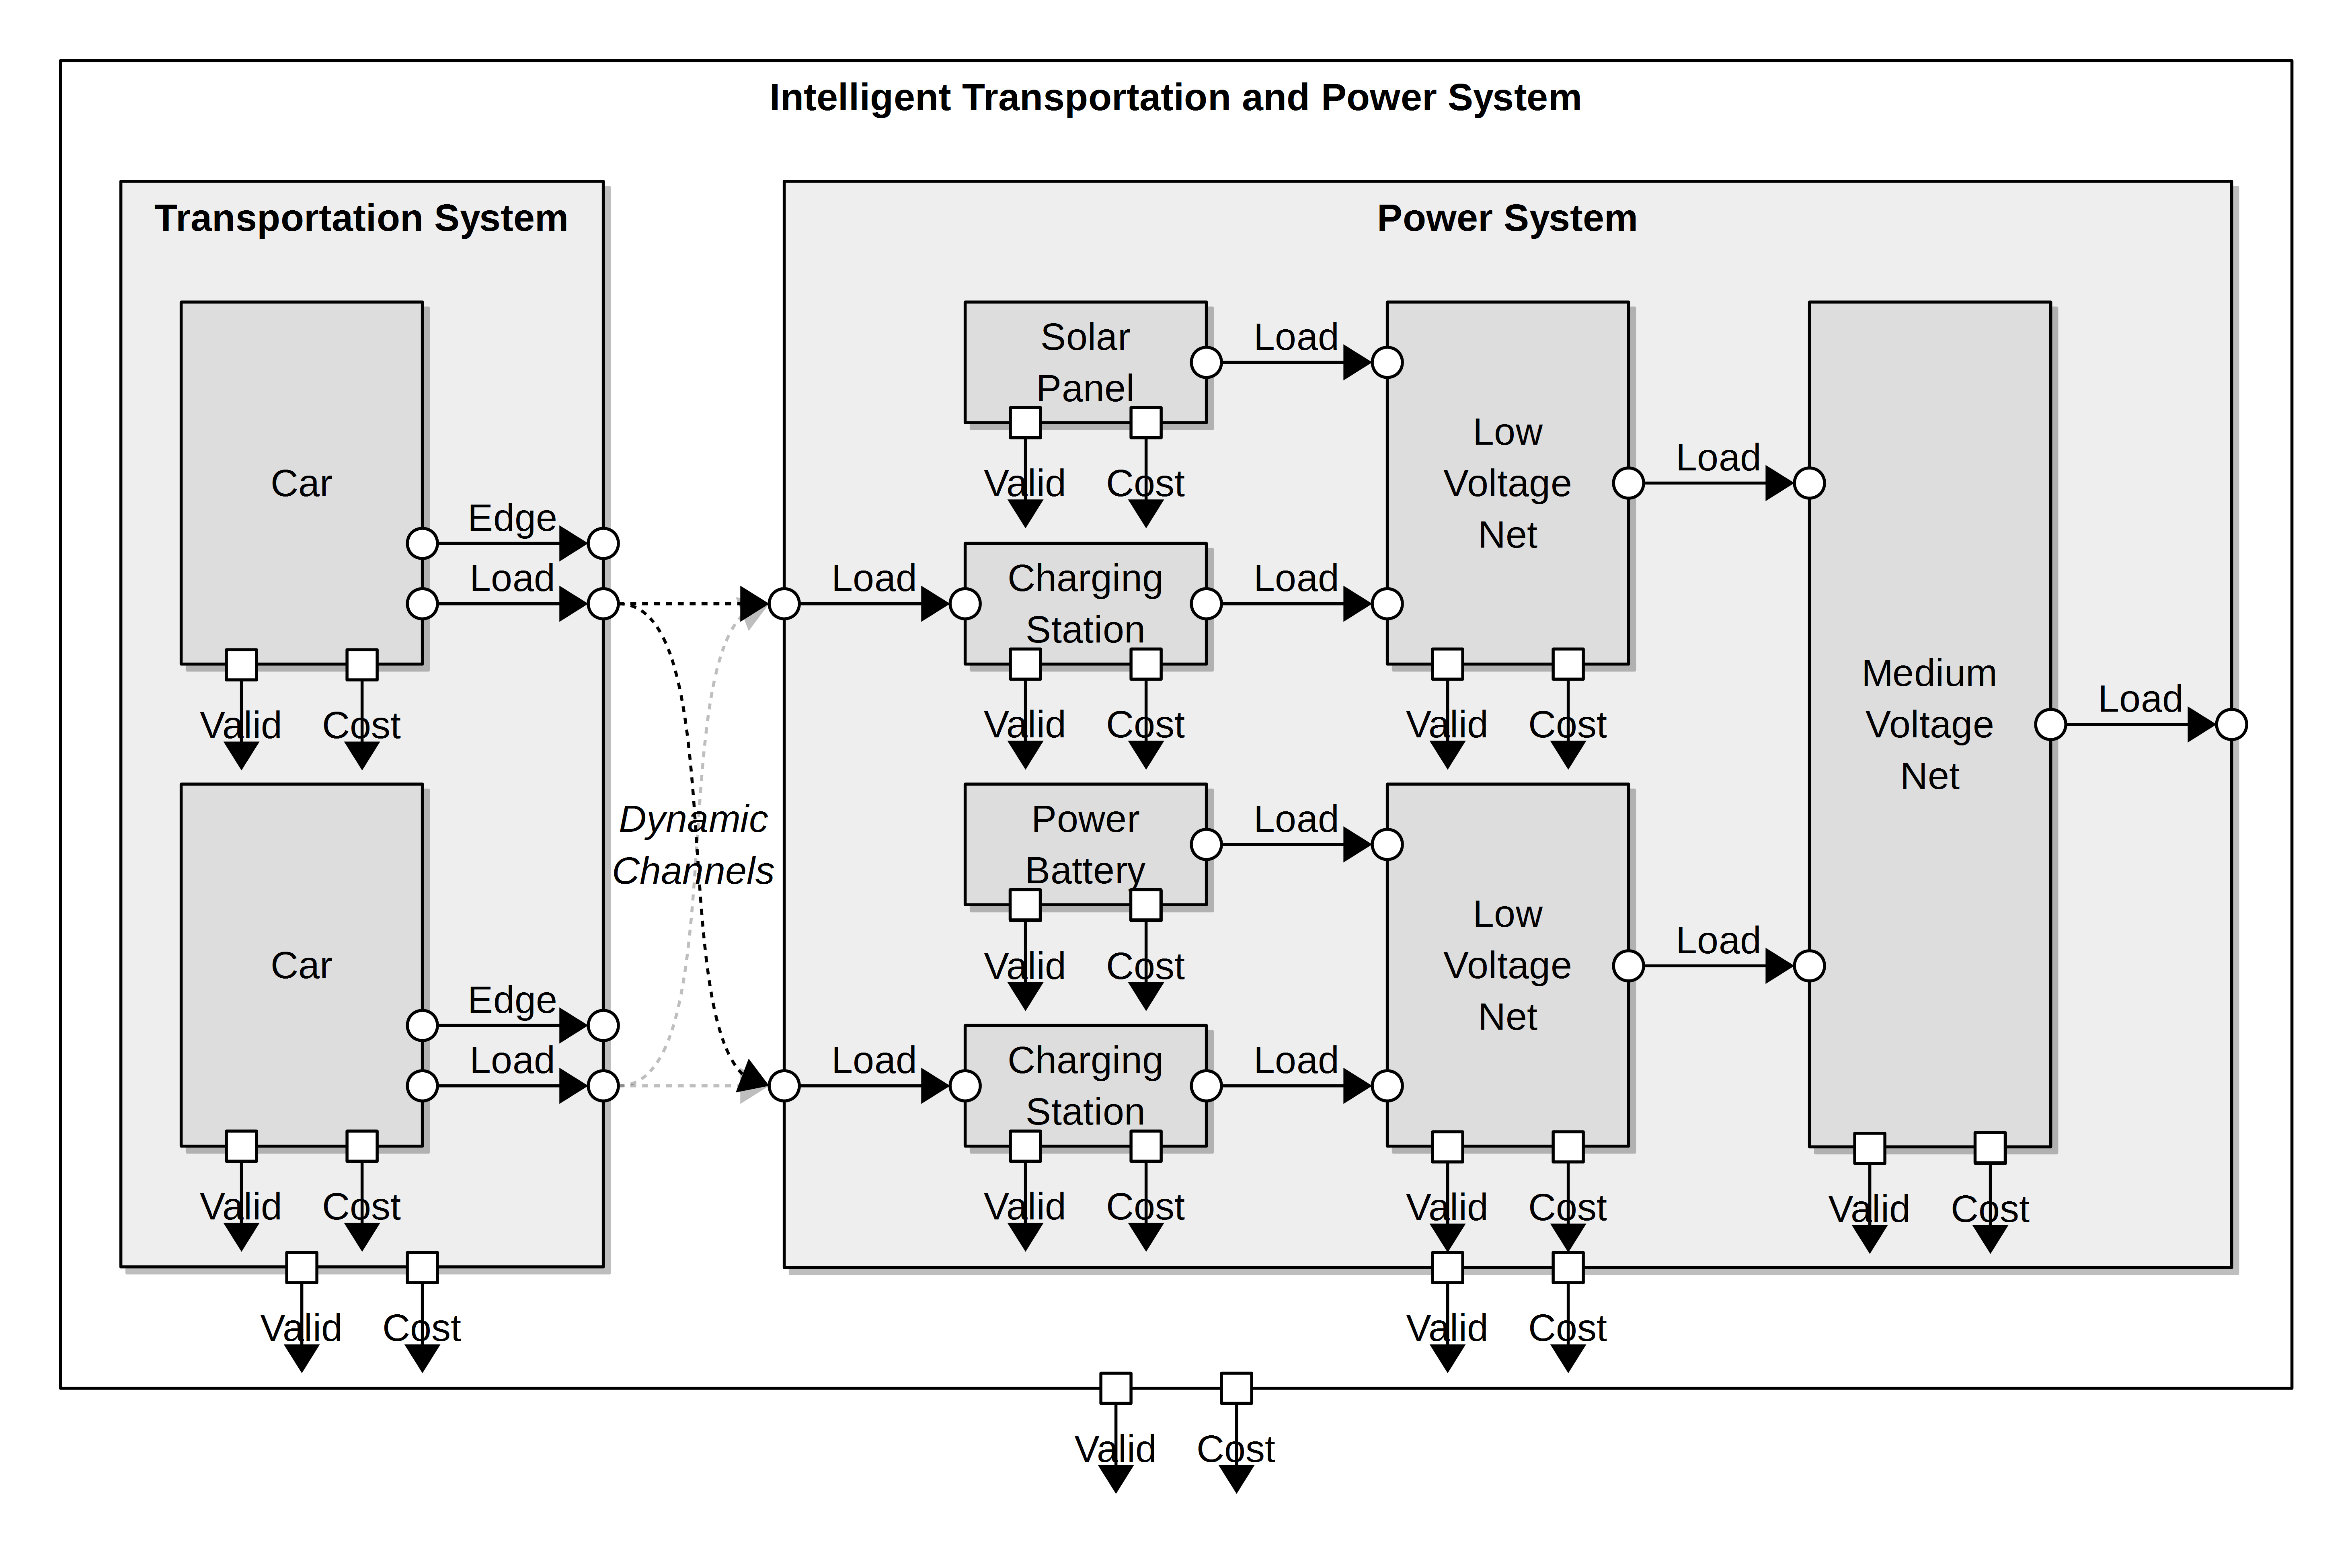
\includegraphics[width=\columnwidth]{../gfx/example.png}
		\caption{Example 1}
		\label{figure:examples_1}
	\end{subfigure}
	\hfill
	\begin{subfigure}{\columnwidth}
		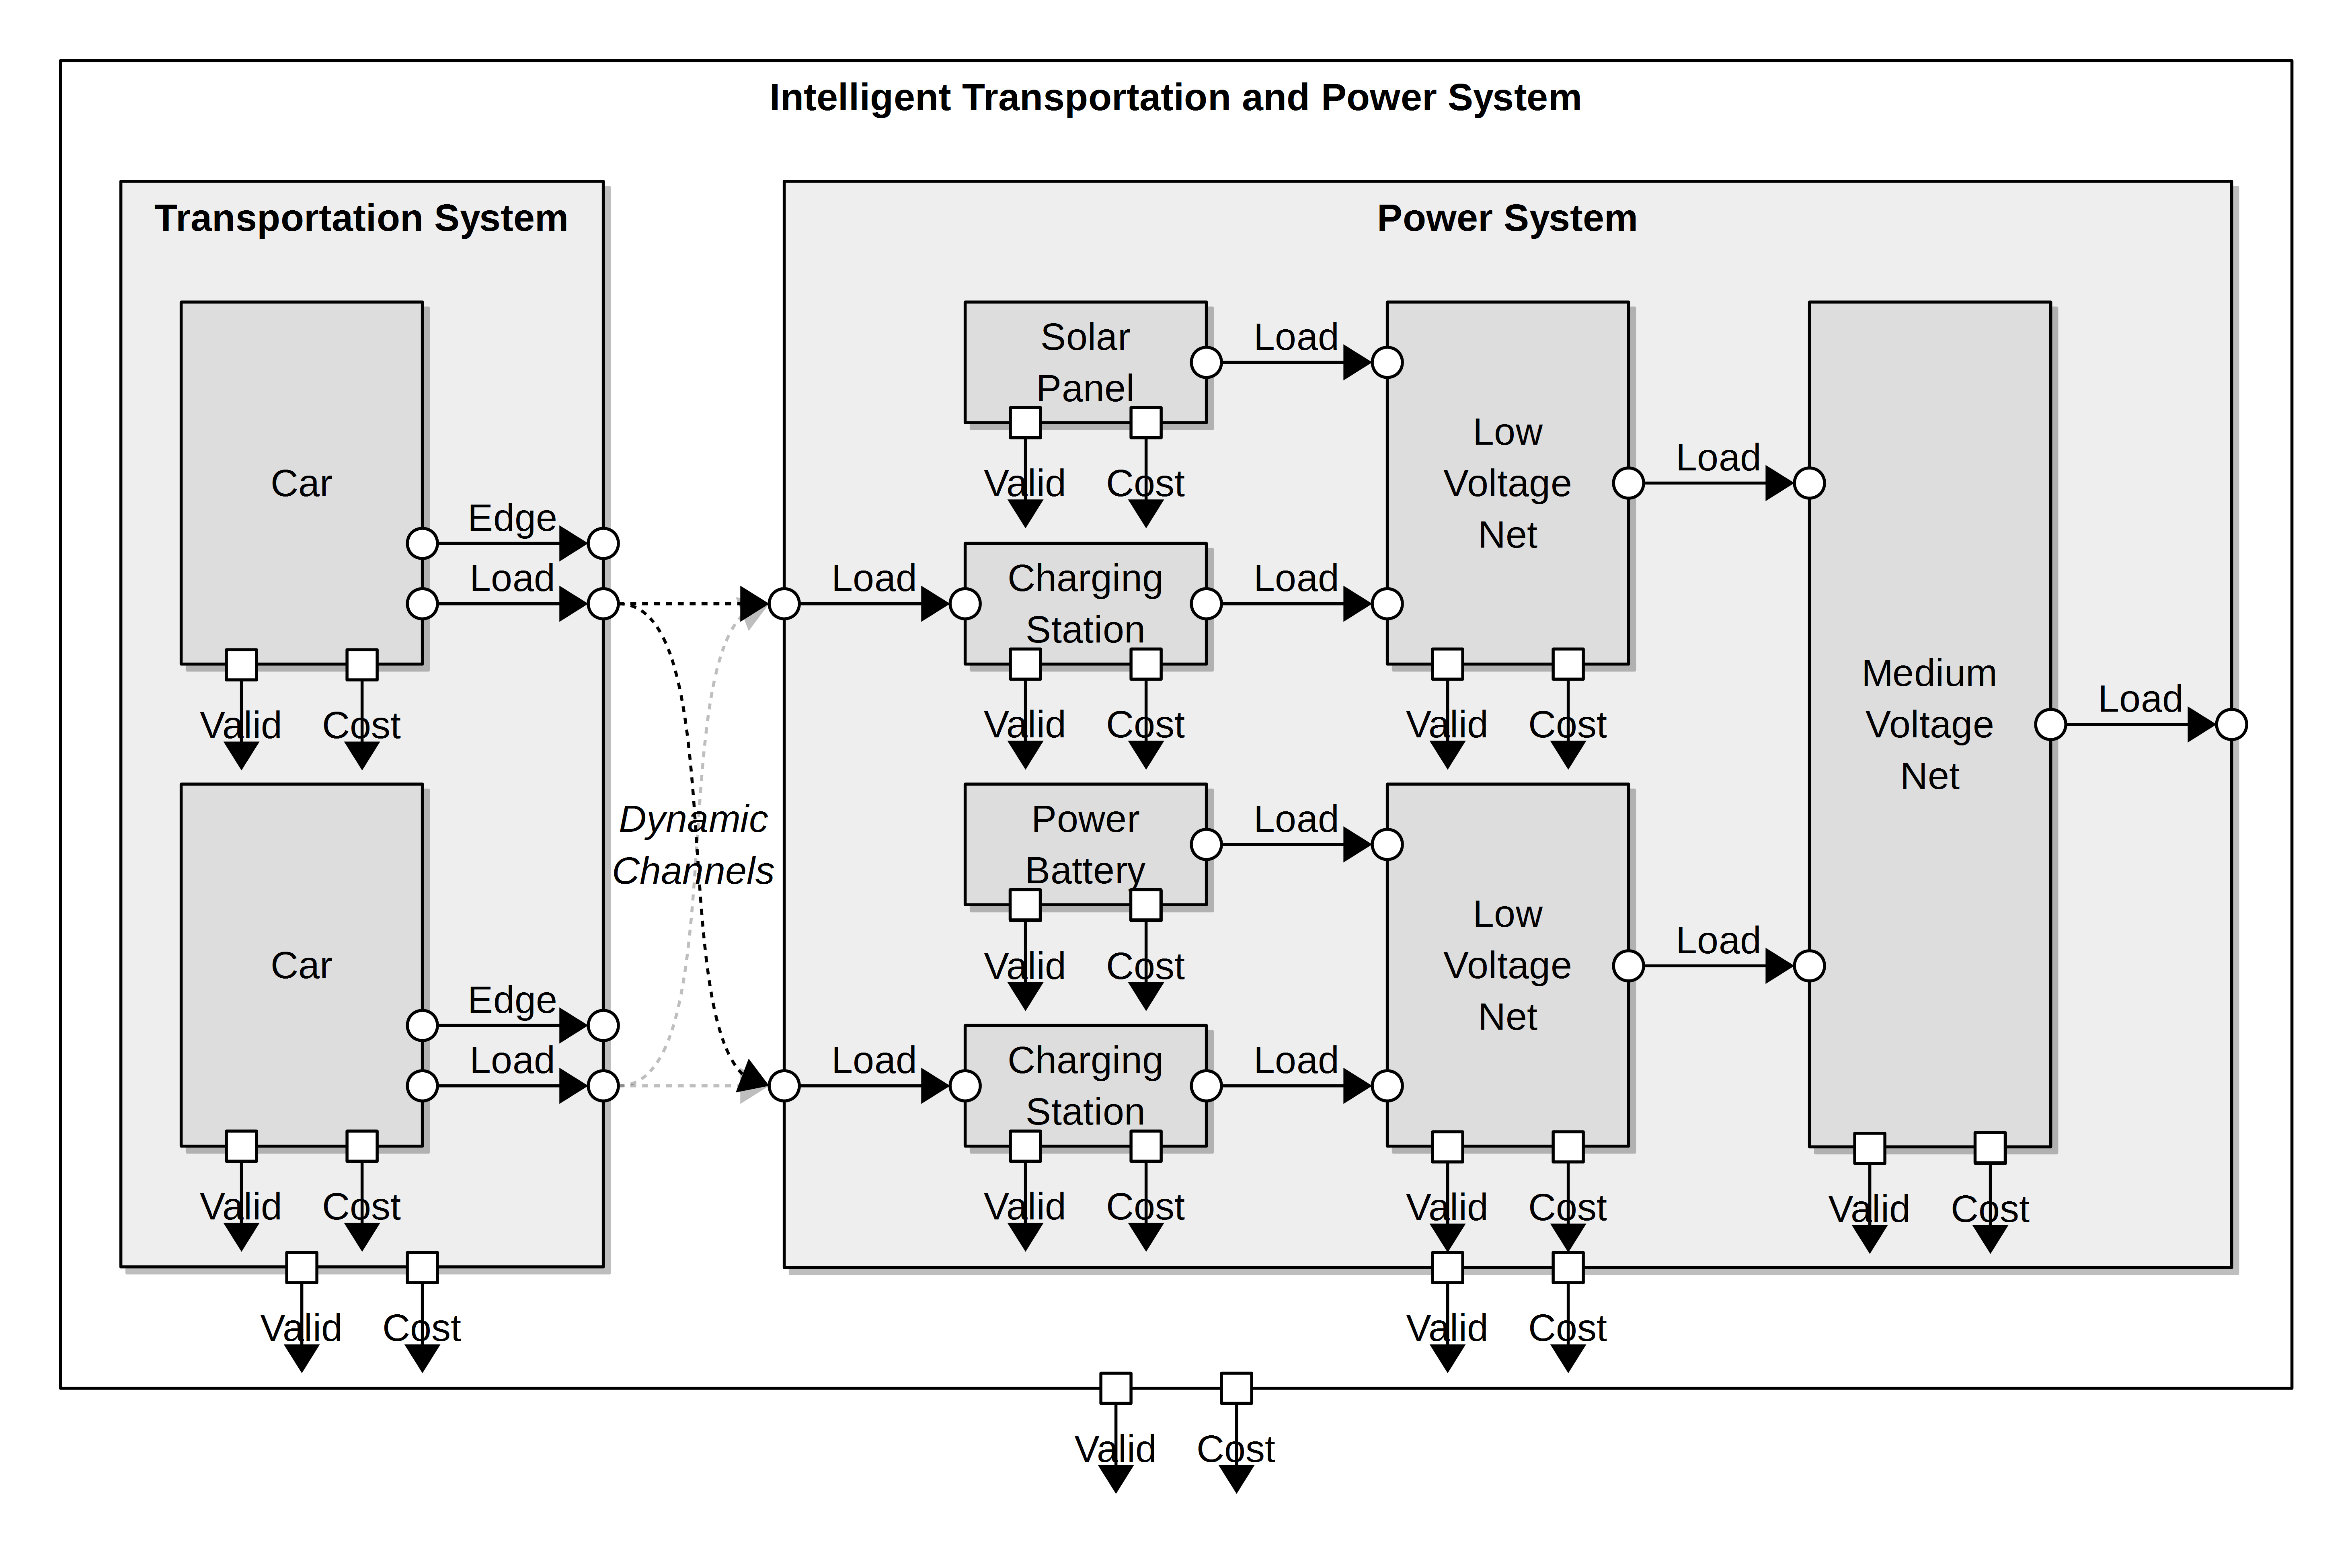
\includegraphics[width=\columnwidth]{../gfx/example.png}
		\caption{Example 2}
		\label{figure:examples_2}
	\end{subfigure}
	
	\begin{subfigure}{\columnwidth}
		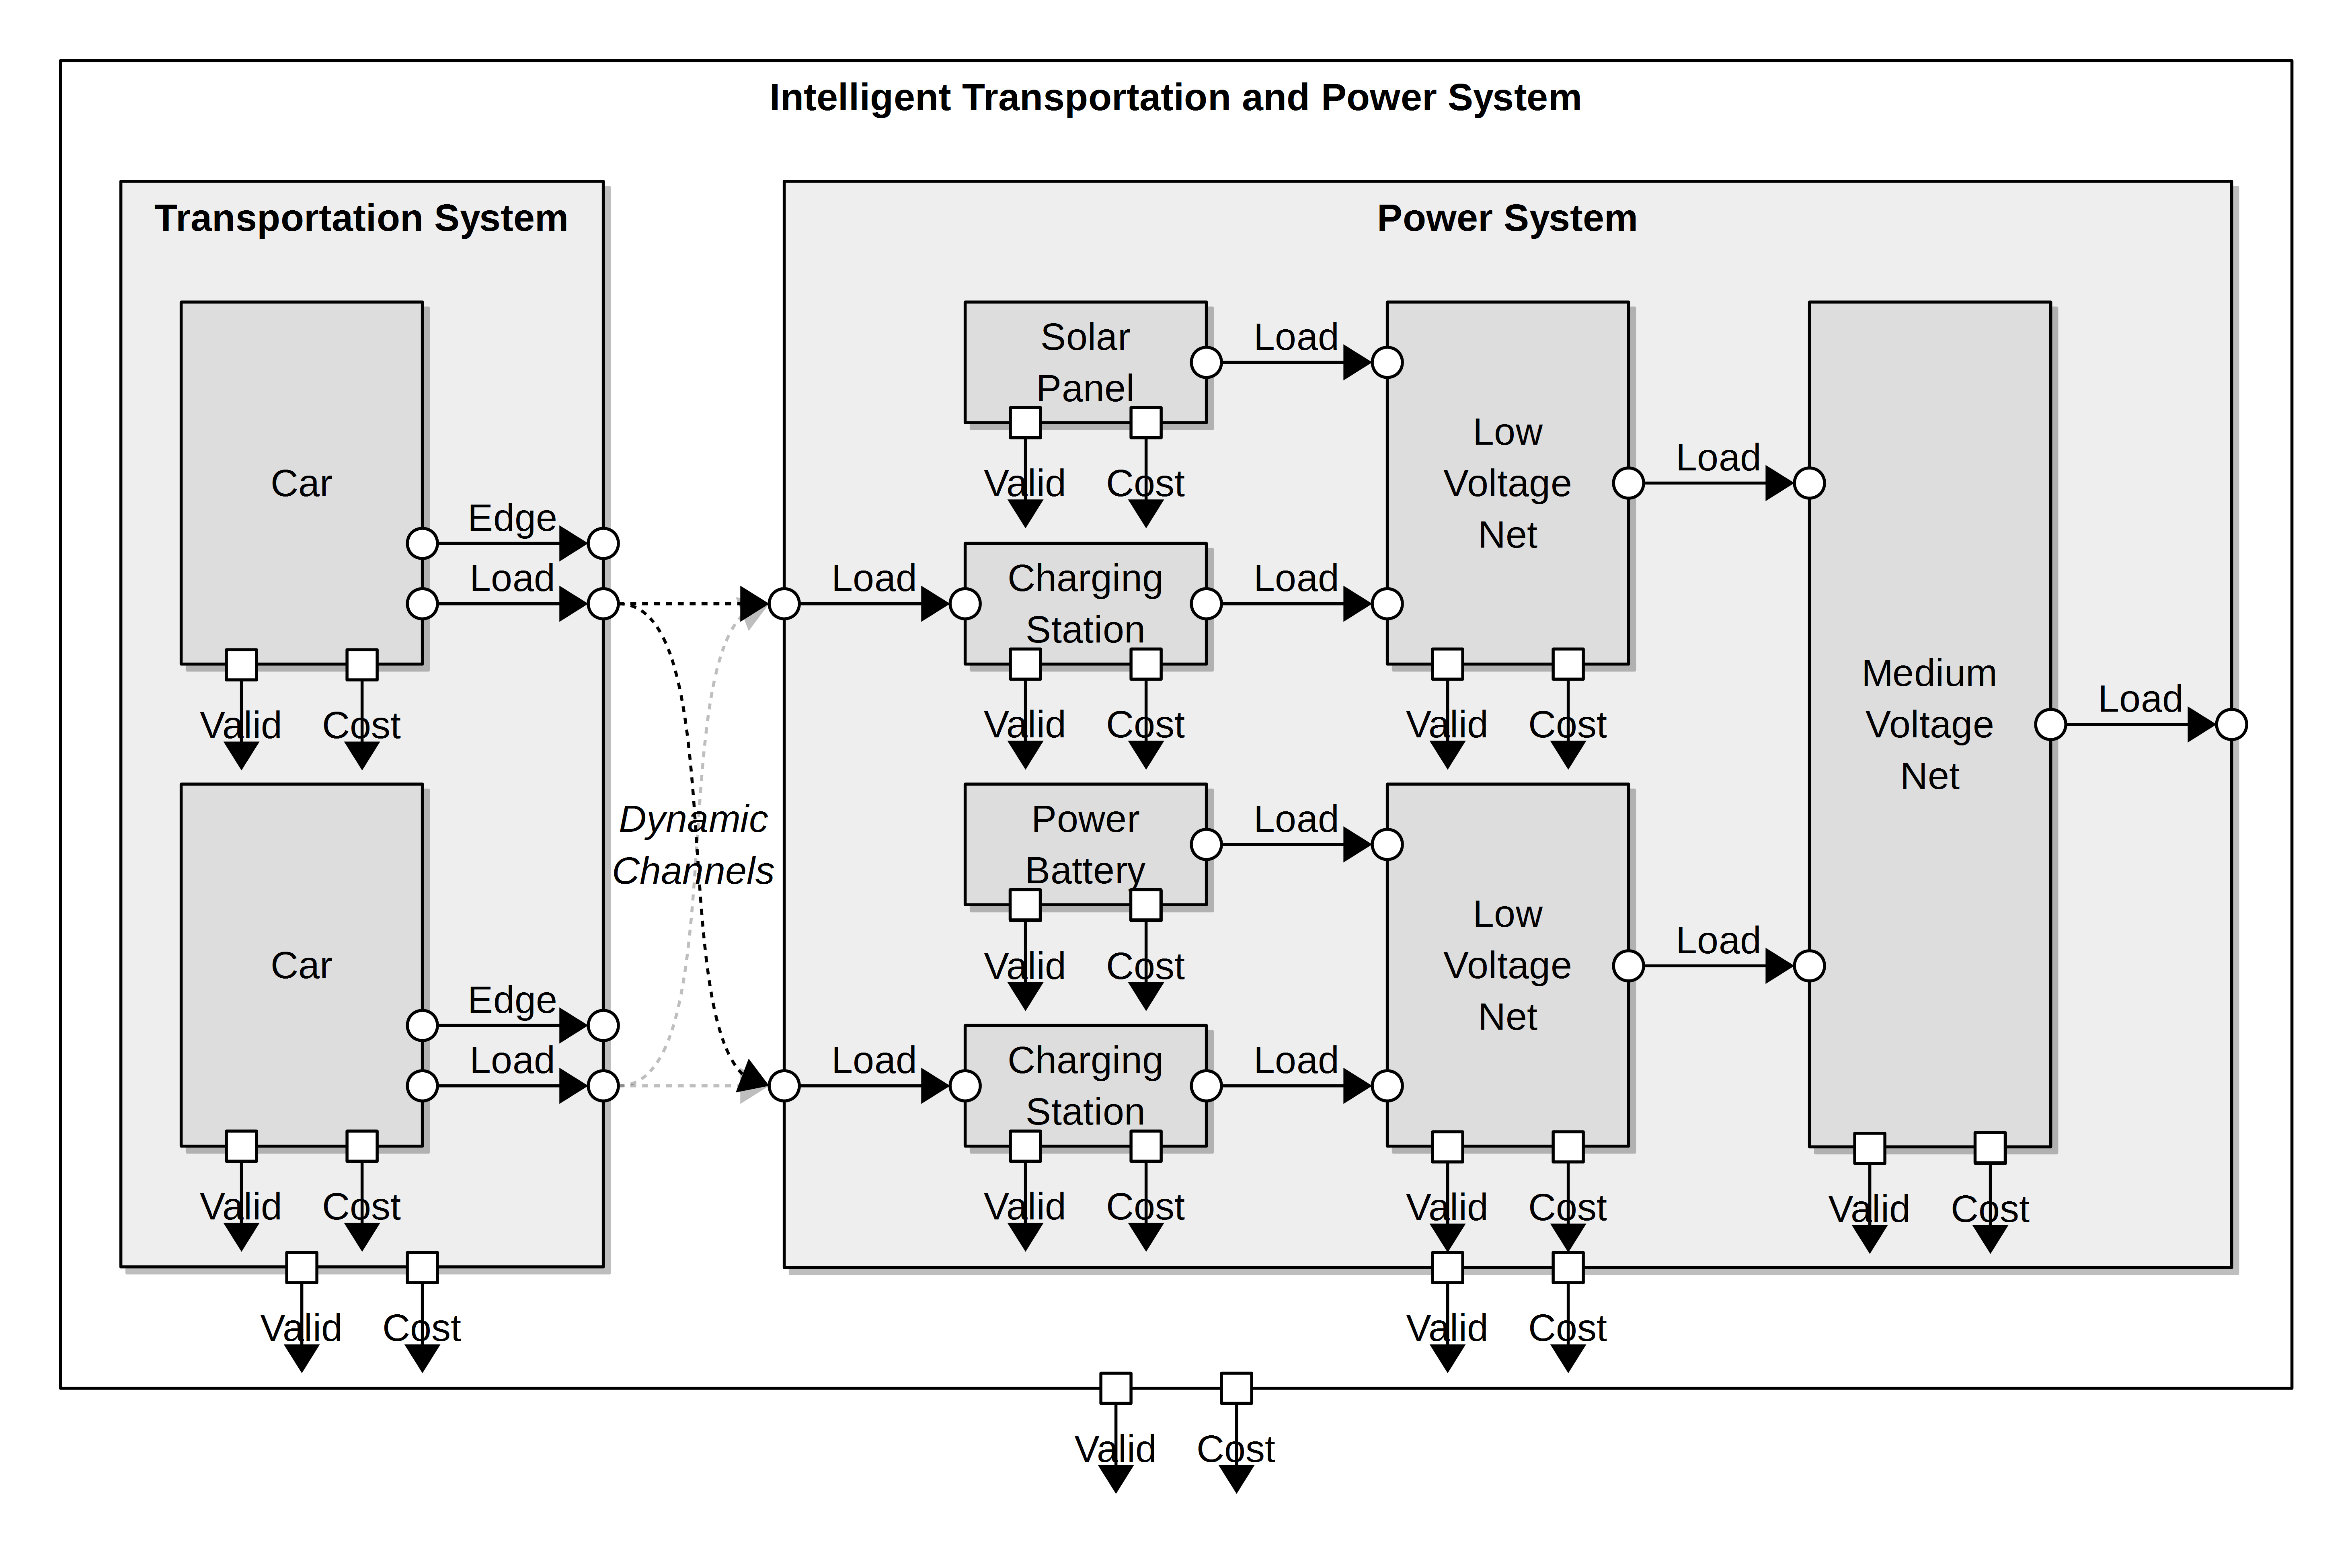
\includegraphics[width=\columnwidth]{../gfx/example.png}
		\caption{Example 3}
		\label{figure:examples_3}
	\end{subfigure}
	\hfill
	\begin{subfigure}{\columnwidth}
		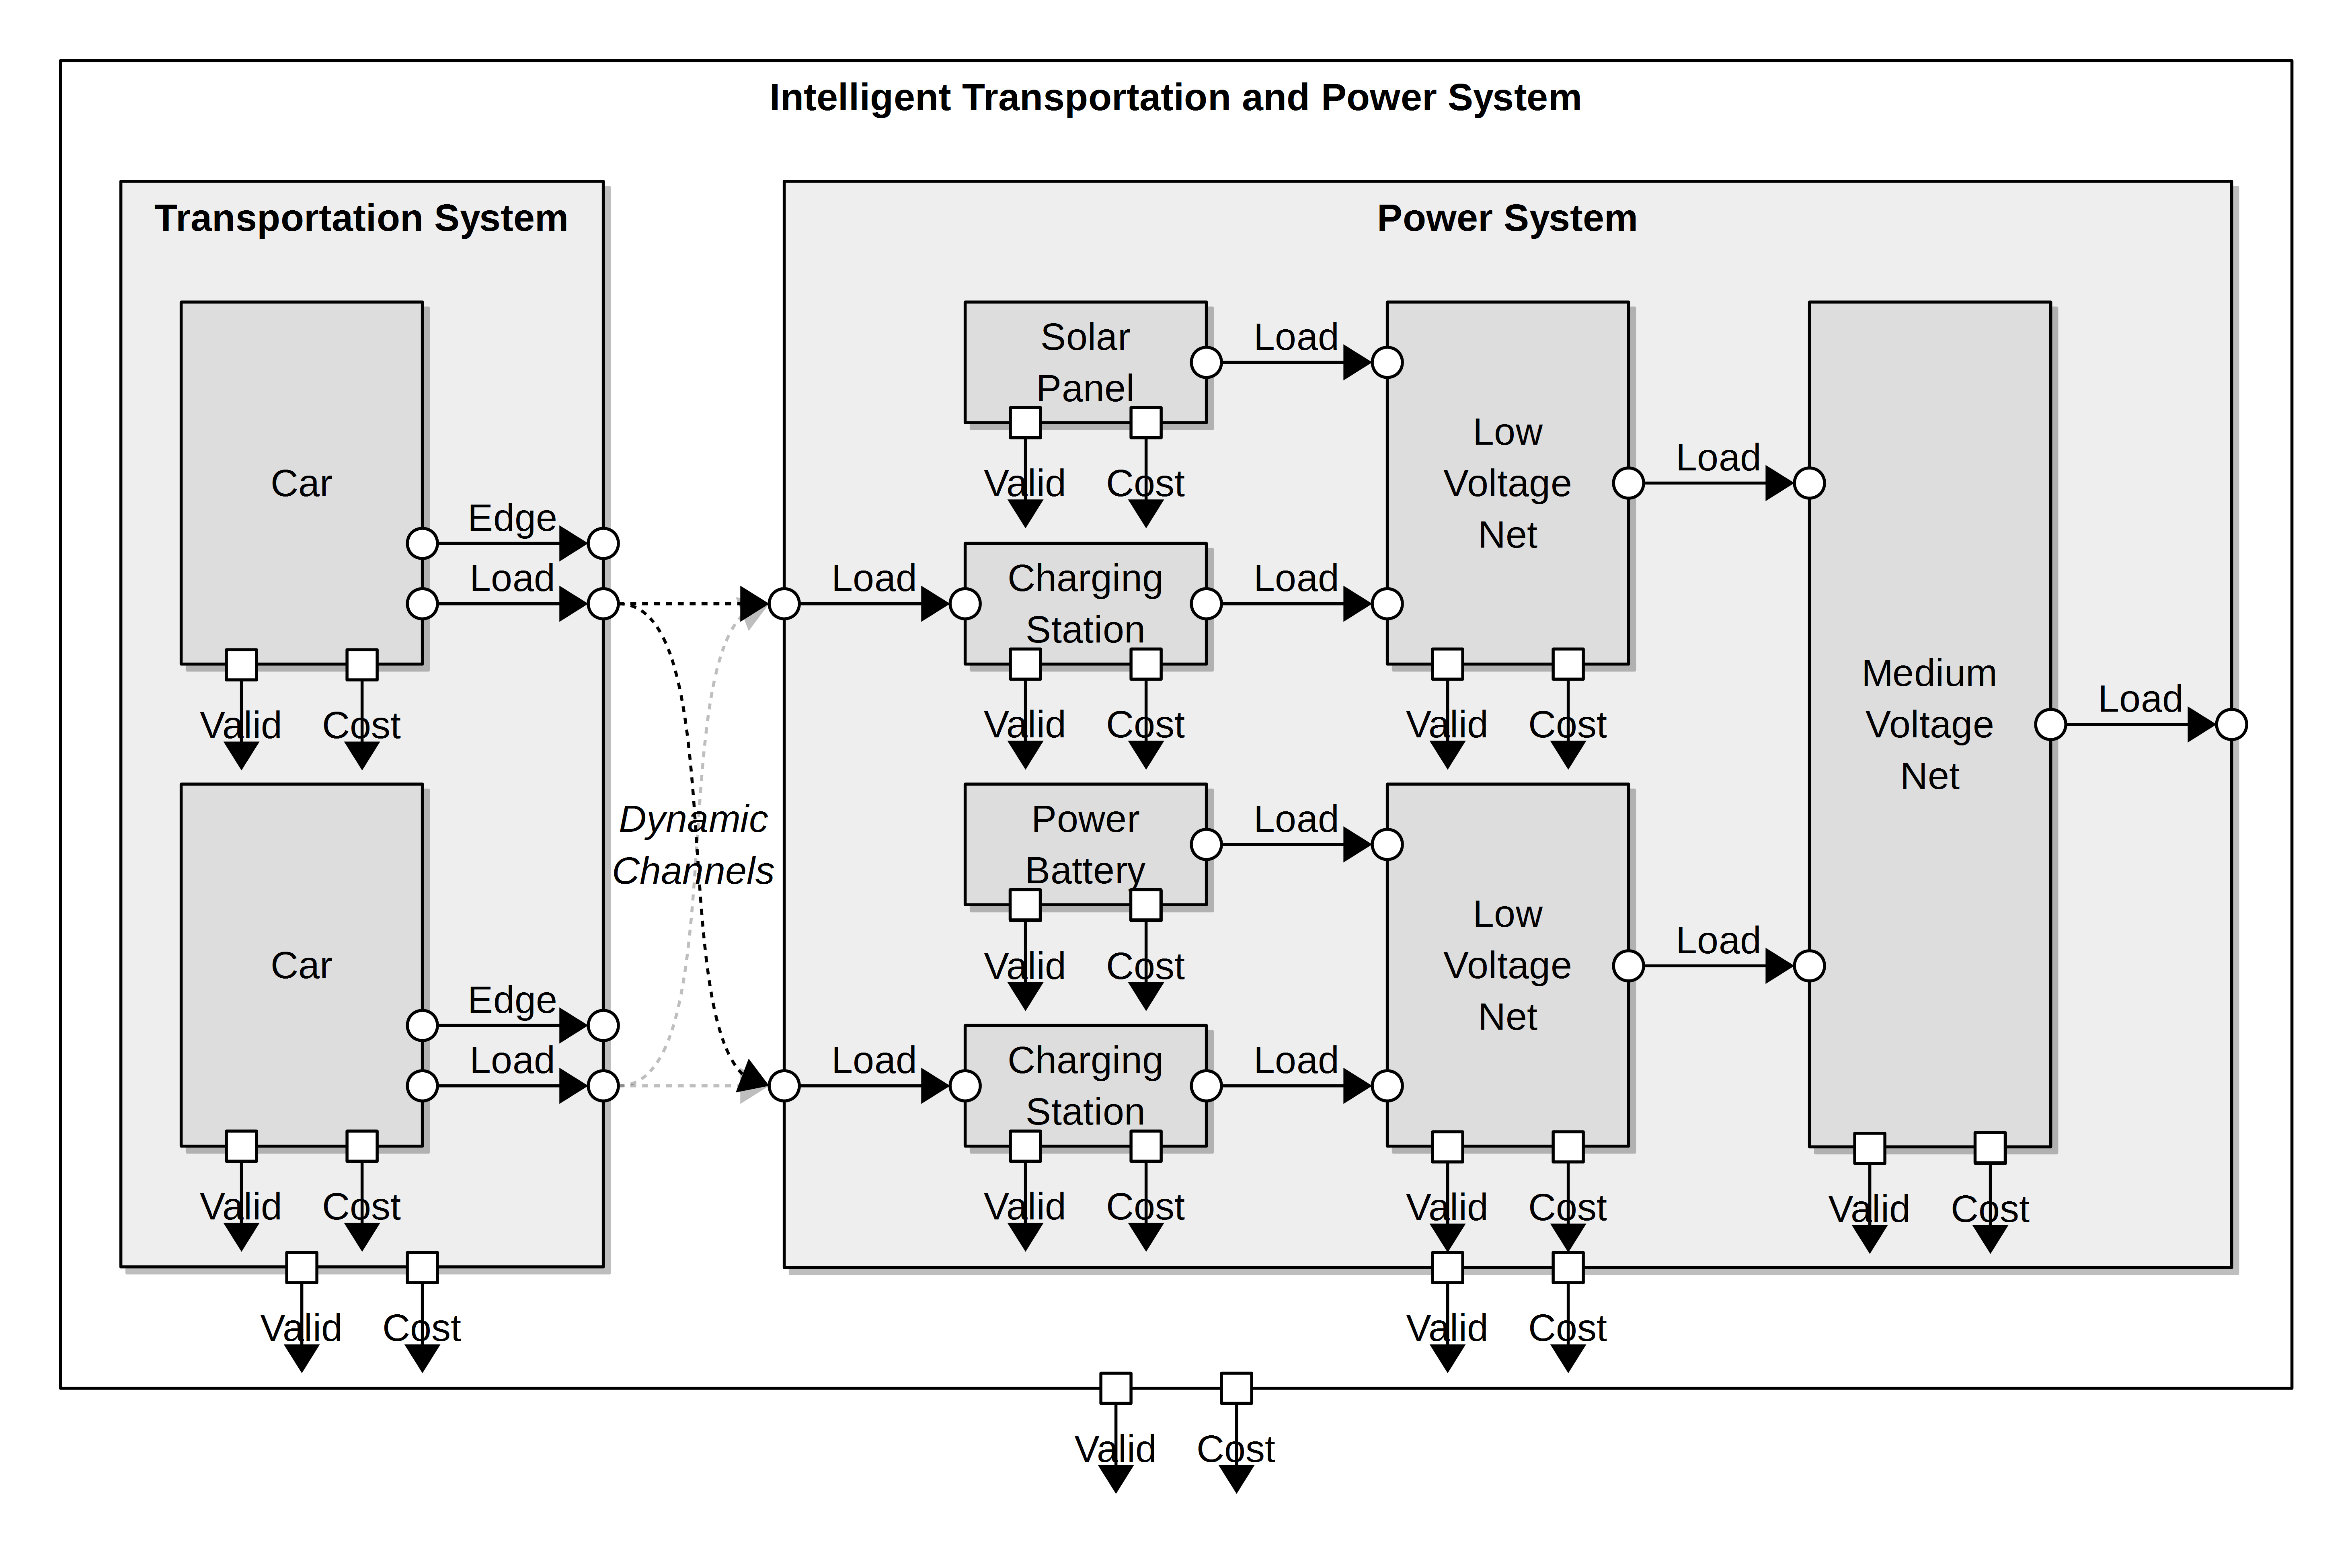
\includegraphics[width=\columnwidth]{../gfx/example.png}
		\caption{Example 4}
		\label{figure:examples_4}
	\end{subfigure}
	
	\caption{Examples.}
	\label{figure:examples}
\end{figure*}